
\documentclass[tikz,border=12pt]{standalone}
\usepackage{pgfplots}
\pgfplotsset{compat=1.18}
\usetikzlibrary{arrows.meta,positioning,fit,calc}
\definecolor{ink}{HTML}{172026}
\definecolor{muted}{HTML}{5F6B73}
\definecolor{line}{HTML}{CBD5E1}
\definecolor{panel}{HTML}{F8FAFC}
\definecolor{bfs}{HTML}{64748B}
\definecolor{spine}{HTML}{0F766E}
\definecolor{hrg}{HTML}{7C3AED}
\definecolor{warn}{HTML}{C2410C}
\definecolor{ok}{HTML}{15803D}
\definecolor{blue}{HTML}{2563EB}
\pgfplotsset{
  every axis/.append style={
    tick label style={font=\small, color=ink},
    label style={font=\small, color=ink},
    title style={font=\bfseries\small, color=ink},
    legend style={font=\footnotesize, draw=none, fill=none},
    grid=major,
    grid style={line!55},
    axis line style={line},
  }
}
\begin{document}

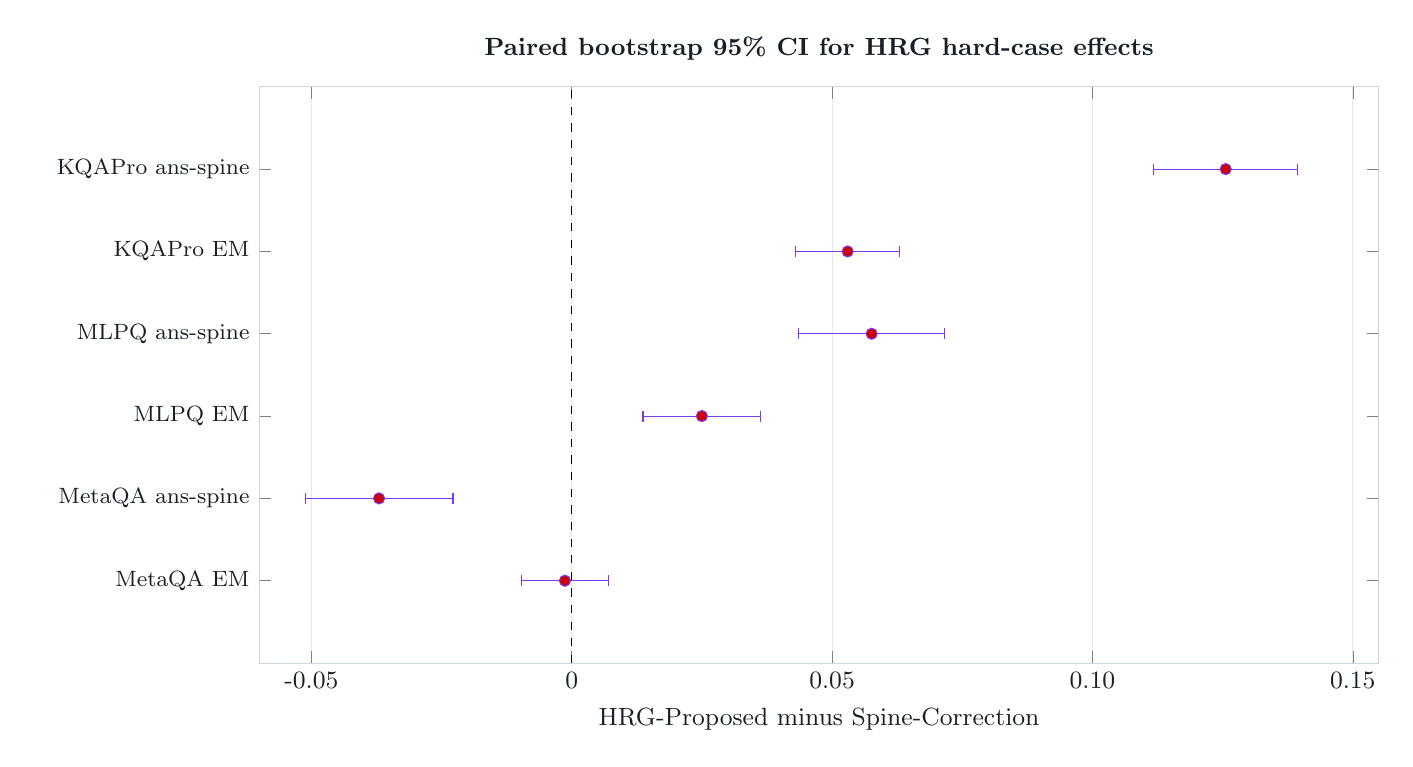
\begin{tikzpicture}
\begin{axis}[
  width=15.8cm,
  height=8.9cm,
  xmin=-0.06, xmax=0.155,
  ymin=0, ymax=7,
  xlabel={HRG-Proposed minus Spine-Correction},
  xtick={-0.05,0,0.05,0.10,0.15},
  xticklabels={-0.05,0,0.05,0.10,0.15},
  ytick={1,2,3,4,5,6},
  yticklabels={MetaQA EM,MetaQA ans-spine,MLPQ EM,MLPQ ans-spine,KQAPro EM,KQAPro ans-spine},
  yticklabel style={font=\footnotesize, align=right, text width=2.7cm},
  title={Paired bootstrap 95\% CI for HRG hard-case effects},
  xmajorgrids=true,
  ymajorgrids=false,
]
\addplot[draw=black, dashed] coordinates {(0,0) (0,7)};
\addplot+[only marks, mark=*, color=hrg, error bars/.cd, x dir=both, x explicit]
coordinates {
  (-0.0013,1) +- (0.0083,0)
  (-0.0370,2) +- (0.0142,0)
  (0.0250,3) +- (0.0113,0)
  (0.0576,4) +- (0.0140,0)
  (0.0530,5) +- (0.0100,0)
  (0.1256,6) +- (0.0138,0)
};
\end{axis}
\end{tikzpicture}

\end{document}
